\chapter{Firewall}\label{fw}
Die Firewall wird in dem Praktikum mit IPTables von Linux realisiert. Dies ermöglicht das Aufstellen von Regeln, welche in Tabellen abgelegt werden, um Verbindungen zwischen zwei Netzen zu kontrollieren. Wenn ein Paket die Firewall erreicht, dann checkt die Firewall sequentiell die einzelnen Regeln. Wenn eine der Regeln zutrifft, dann wird das Paket entweder mittels ACCEPT akzeptiert oder mittels DROP fallengelassen. Bei ACCEPT wird das Paket weiter gereicht und bei DROP wird das Paket einfach fallen gelassen und der Zielrechner erhält nicht das Paket. Wenn keine Regel zutrifft, dann wird die Default Policy angewandt. Diese kann wiederum auf DROP und ACCEPT gesetzt sein.
\begin{figure}
	\centering
		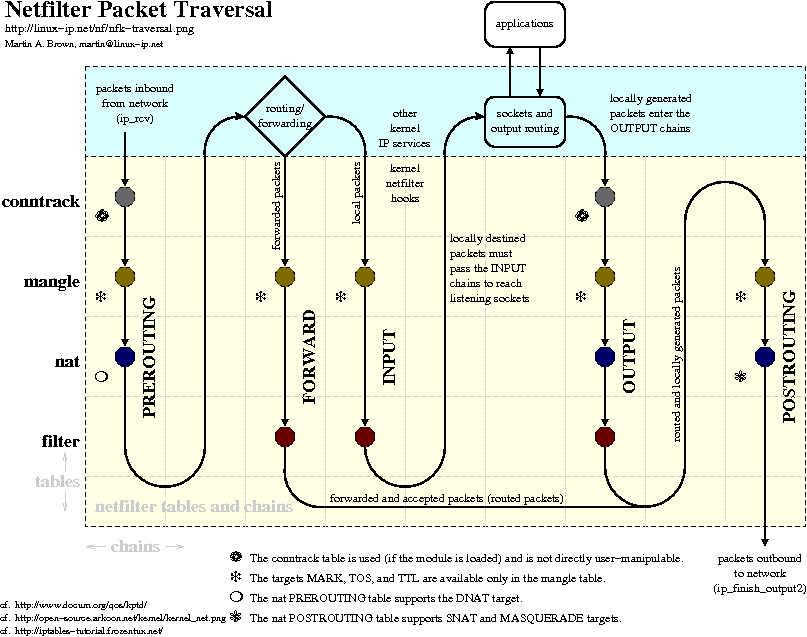
\includegraphics[width=1.00\textwidth]{figures/firewall_uebersicht.PNG}
	\caption{Firewall Übersicht \cite{linux-ip}}
	\label{fig:firewall_uebersicht}
\end{figure}
In Abbildung \ref{fig:firewall_uebersicht} ist zu sehen, dass es verschiedene Tabellen gibt. Je nachdem ob das Paket weitergeleitet wird oder einen lokalen Prozess als Ziel hat, werden die zuständigen Tabellen geprüft. Die Tabellen mit den Regeln werden auch Ketten (Chains) genannt. Folgend eine kurze Auflistung der vorhandenen Ketten und wann welche geprüft werden.
\begin{itemize}
	\item PREROUTING \\
	Hier landen Pakete bevor entschieden worden ist, ob das Paket weitergeleitet wird oder einen lokalen Prozess als Ziel hat. Somit können hier Port Weiterleitungen eingetragen werden.
	\item POSTROUTING \\
	Ganz zum Schluss, wenn schon alle vorherigen Entscheidungen getroffen worden sind. Dann durchlaufen alle Pakete noch die Postrouting Kette.
	\item FORWARD \\
	Hierbei handelt es sich um ein Paket, welches weitergeleitet wird.
	\item INPUT \\
	Das Paket hat einen lokalen Prozess als Ziel, welcher sich auf dem Rechner, auf dem die Firewall läuft, befindet.
	\item OUTPUT \\
	Hierbei handelt es sich um ein Paket, welches von einem lokalen Prozess abgesendet wird.
\end{itemize}
Die Regeln zur Beurteilung eines Paketes beschränken sich auf die OSI-Schichten 3 und 4. Somit hat man Zugriff auf die Übertragungsflags, IP-Adressen, Ports und die zugehörigen Netzwerkinterfaces. IPTables ermöglicht verbindungsorientierte Paketfilter, somit kann zum Beispiel überprüft werden ob eine Verbindung related ist, dass heißt es wird eine Unterverbindung aufgebaut, wo schon eine Verbindung zwischen den Rechnern besteht. Diese neue Verbindung hat in der Regel einen anderen Port. Dieser wird von vielen Programmen zufällig bestimmt und somit muss die Firewall Verbindungsaufbau zwischen "`New"' und "`Related"' unterscheiden können. Des Weiteren ermöglicht IPTables eine NAT mit Masquerade Funktion. Das bedeutet es versteckt die Rechner von einem Netzwerk vor dem anderen Netzwerk.

\section{Stateful - Stateless}
Es gibt grundlegend zwei verschiedene Arten von Firewalls, darunter fallen stateful- und stateless Firewalls. Eine stateless Firewall kann nur Pakete filtern anhand der Paketinformationen und kann somit keine weiteren Daten zur Beurteilung eines Paketes heranziehen. Eine stateful Firewall hingegen kann Daten zu bestehenden Verbindungen speichern. Dies ermöglicht z.B., dass neue Verbindungen aus einer schon bestehenden Verbindung aufgebaut werden können, wobei der Port ein anderer sein kann. Somit kann eine neue Verbindung von einer neuen Unterverbindung unterschieden werden. Ebenso kann eine stateful Firewall effektiver DoS Angriffe abwehren, weil sie zum Beispiel speichern kann wie häufig von einem Rechner eine neue Verbindung aufgebaut wurde und kann somit nach einer bestimmten Anzahl von Verbindungen alle Pakete fallen lassen. Allgemein sind stateless Firewalls schneller und einfacher zu handhaben, bieten hingegen nicht die Möglichkeiten einer stateful Firewall. IPTables ist eine stateful Firewall und bietet somit mehrere States anhand dessen die Filterregeln aufgestellt werden können.

\subsection{IPTables - States}
Wichtiger Bestandteil einer Filterregel sind die States. Folgend ist eine kurze Auflistung der verschiedenen States und wann diese einem Paket zugeordnet werden.
\begin{itemize}
	\item NEW \\
	Hierbei handelt es sich um ein Paket, welches eine neue Verbindung aufbaut. Somit ist es immer das erste Paket einer Verbindung.
	\item ESTABLISHED \\
	Hierbei handelt es sich um Pakete welche einer bestehenden Verbindung angehören.
	\item RELATED \\
	Hierbei handelt es sich um ein Paket welches eine neue Verbindung aufbaut. Jedoch besteht schon eine weitere Verbindung zwischen den Rechnern.
	\item INVALID \\
	Hierbei handelt es sich um Pakete, deren State nicht erkannt werden kann.
	\item UNTRACKED \\
	Hierbei handelt es sich um Verbindungen welche nicht Stateful gespeichert werden. Dies kann mittels einer "`raw table"' zu bestimmten Verbindungen zugewiesen werden. Dann sind alle Pakete dieser Verbindung mit dem State UNTRACKED.
\end{itemize}

\section{Anforderungen}
Im Praktikumsaufbau gibt es zwei Firewalls. Hierbei handelt es sich um eine äußere Firewall, welche wie in Abbildung \ref{fig:netzplan} zu erkennen die Verbindungen zwischen der DMZ und dem Internet regelt. Die Rechner aus der DMZ werden vor Rechnern aus dem Internet versteckt. Die innere Firewall hat dabei dieselben Aufgaben nur ist sie zwischen der DMZ und dem Firmennetzwerk platziert.

\subsection{Äußere Firewall (FW1)}
\begin{itemize}
\item Masquerading von der DMZ zum Internet.
\item Rechner aus der DMZ sollen weiterhin alle Verbindung zum Internet aufbauen können.
\item Der Webserver aus der DMZ soll von dem Internet über die üblichen Ports erreichbar sein. Darunter fallen folgende Ports. 80(HTTP), 443(HTTPS), 25(SMTP), 587(SMTP), 465(SMTPS), 993(IMAPS), 995(POP3S), 143(IMAP), 110(POP3), 53(DNS)
\item Die interne Firewall muss erreichbar sein für das VPN. Somit müssen folgende Ports auf die innere Firewall weitergeleitet werden. 1195(VPN: Client to Lan), 1194(VPN: Lan to Lan)
\end{itemize}

\subsection{Innere Firewall (FW2)}
\begin{itemize}
\item Masquerading von dem Firmennetz zur DMZ. Somit dürfen die IP Adressen der Rechner aus dem Firmennetz in der DMZ nicht erkennbar sein, sondern als IP Adresse ist die der Firewall zu sehen.
\item Es dürfen keine neuen Verbindungen von der DMZ in das interne Firmennetz aufgebaut werden.
\item Rechner aus dem Firmen internen Netzwerk dürfen neue Verbindungen zur DMZ und dem Internet aufbauen.
\item Auf der inneren Firewall läuft der VPN Dienst und dieser muss aus dem Internet erreichbar sein.
\end{itemize}

\section{Implementierung}
Damit die Praktikumsaufgabe reibungslos bearbeitet werden kann, wurde zu Anfang das NAT/Masquerading eingerichtet. Daraufhin wurde das VPN eingerichtet und getestet. Und sobald alle Funktionalitäten geprüft waren, wurde der Paketfilter eingerichtet. Durch diese Reihenfolge konnte sichergestellt werden, dass der Paketfilter von der Firewall nicht die Funktionalität des VPN Dienstes stört.

IPTables speichert seine Tabelleneinträge nur im Arbeitsspeicher, deswegen sind die Einträge welche hinzugefügt werden nach einem Neustart des Rechners wieder verschwunden. Damit die Einträge gespeichert werden, müssen diese mittels dem iptables-save Befehl in eine Datei gespeichert werden.
\begin{lstlisting}
iptables-save > /etc/iptables.rules
\end{lstlisting}
Durch diesen Befehl werden alle IPTables Einträge in /etc/iptables.rules gespeichert. Damit nach einem Neustart diese Einträge auch geladen werden, muss unter /etc/network/if-pre-up.d/ ein Skript erstellt werden, welches die gespeicherten Einträge mittels iptables-restore aus der Datei lädt. Debian speichert ebenfalls ausführbare Skripte im if-pre-up.d Ordner, die vor dem Start der Netzwerkdienste ausgeführt werden müssen. Unser Skript zum laden der IPTables Regeln sieht wie folgt aus:
\begin{lstlisting}[caption={/etc/network/if-pre-up.d/iptables}]
iptables-restore < /etc/iptables.rules
\end{lstlisting}
Mit dem Befehl \texttt{chmod +x} wurde bei dem Skript das ausführbar Flag gesetzt. Somit werden die IPTables Regeln aus der Datei /etc/iptables.rules bei jedem Start des Rechners geladen. Dadurch können die IPTables mit dem normalen \texttt{iptables} Befehlen eingerichtet werden und durch den \texttt{iptables-save} Befehl gespeichert werden. Die Konfiguration der Firewall durch aufrufen des Skripts, wurde auf beiden Firewalls so eingerichtet.

\subsection{Default Policy}
In dem Praktikumsszenario handelt es sich um ein Firmennetzwerk, deswegen wurde die Default-Policy auf DROP gesetzt. Mit folgenden Befehlen:
\begin{lstlisting}[caption={Befehle für Default Policy}]
iptables -P FORWARD DROP
iptables -P OUTPUT DROP
iptables -P INPUT DROP
\end{lstlisting}
Hierbei muss wenn ein neuer Dienst eingerichtet wird, dieser explizit in der Firewall eingetragen werden, damit dieser auch Problemlos funktioniert.

\subsection{ICMP}
Das Internet Control Message Protkoll dient dazu, Informationen und Fehlermeldungen über das Netzwerk zu übertragen. Wenn zum Beispiel ein Paket verworfen wird, dann kann dies mittels einer ICMP Nachricht demjenigen der versucht eine Verbindung aufzubauen mitgeteilt werden. Diese Informationen sind zur Wartung und zum Testen eines Systems sehr praktisch. Sie können aber auch für einen Angreifer interessant sein. Auf diesen Rechnern wurden diese Pakete erlaubt, damit mittels \texttt{ping} getestet werden kann, welche Rechner erreichbar sind. Somit wurden folgende Regeln für die Input Kette erstellt.
\lstinputlisting[
    firstline=9,
    lastline=9,
    label = fw:fw1_iptables_icmp,
    caption={FW1 iptables.rules - Ausschnitt ICMP Paketfilter}
]{code/fw1_iptables.rules}
Dasselbe wurde auf der zweiten Firewall auch eingerichtet. Somit sind die Firewall Rechner weiterhin pingbar. Man kann diesen Filter auch entfernen, wenn man sich sicher ist, dass alles in Ordnung läuft. Dadurch gewinnt man nochmals einen kleinen Grad an Sicherheit. Jedoch erschwert es bei auftretenden Fehlern die Fehlersuche. Für dieses Praktikum war die erleichterte Fehlersuche der Hauptgrund für das Erlauben dieser Pakete.

\subsection{NAT / Masquerading}
Das Einrichten von Masquerading erfolgte auf beiden Firewall Rechnern gleich, da diese Funktionalität auf beiden die selbe ist. Die Netzwerkschnittstelle "`eth0"' ist mit dem Netzwerk verbunden, welches versteckt werden soll. Wobei "`eth1"' mit dem Netzwerk verbunden ist, welchem nicht zu vertrauen ist. Das ist einmal die DMZ von dem firmeninternen Netzwerk und das Internet gesehen von der DMZ. \\
Als erstes musste unter /etc/sysctl.config das Forwarding der Pakete aktiviert werden. Dies erfolgte mit dem ändern des ipv4 forward Flags.
\begin{lstlisting}[caption={/etc/sysctl.config}]
net.ipv4.ip_forward=1
\end{lstlisting}
Somit ist das weiterleiten der Pakete ermöglicht. Das Masquerading wird dann mittels IPTables realisiert. Dafür muss folgender Eintrag hinzugefügt werden.
\begin{lstlisting}
iptables -t nat -A POSTROUTING -o eth1 -j MASQUERADE
\end{lstlisting}
Durch diesen Eintrag wird "`eth1"' als Output Netzwerkinterface für das Masquerading verwendet. Dieser Eintrag wird in die dafür zuständige NAT Tabelle eingetragen. Dies ist mittels -t nat zu erkennen.

\subsection{Implementierung FW1 (DMZ - Internet)}
Diese Firewall regelt die Verbindung zwischen der DMZ und dem Internet. Somit ist es wichtig, dass Pakete welche an bestimmten Ports ankommen, auch an den zutreffenden Server weitergeleitet werden. In diesem Praktikum ist das der Server mit dem DNS-Namen "`srv1.firma-a.f223"' mit der IP-Adresse "`192.168.40.1"'. Das bedeutet es müssen zuerst die Pakete welche an die Firewall ankommen in der Prerouting Kette weitergeleitet werden. In der Auflistung \ref{fw:fw1_iptables_prerouting} sind Einträge für die Nat Tabelle in der Kette Prerouting zu erkennen. Es wird anhand des ankommenden Netzwerkinterfaces und Port entschieden ob das Paket weitergeleitet wird an den Webserver. Hier wurden alle relevanten Ports eingetragen.
\lstinputlisting[
    firstline=35,
    lastline=48,
    label = fw:fw1_iptables_prerouting,
    caption={FW1 iptables.rules - NAT Prerouting}
]{code/fw1_iptables.rules}
Ebenso werden die udp Pakete welche für das VPN zuständig sind, an die innere Firewall weitergeleitet mit der IP-Adresse "192.168.40.250". Diese Pakete welche weitergeleitet werden, kommen somit an die Paketfilter Regeln an der Kette Forward. Damit diese dort nicht einfach verworfen werden, müssen die Ports in dieser Kette ebenfalls eingetragen werden. Dies ist in folgenden Auflistung zu sehen.
\lstinputlisting[
    firstline=10,
    lastline=24,
    label = fw:fw1_iptables_forward,
    caption={FW1 iptables.rules - Paketfilter Forward}
]{code/fw1_iptables.rules}
Somit werden alle Pakete akzeptiert, welche den state "`NEW"' haben und aus dem Internet auf den Webserver weitergeleitet werden. Das sind die Zeilen 3 bis 13 in der Auflistung \ref{fw:fw1_iptables_forward}. Die Zeilen 14 und 15 sind wiederum für die Pakete des VPN Dienstes zuständig. Die erste Zeile erlaubt Pakete von der DMZ zum Internet. Die zweite Zeile erlaubt bei schon aufgebauten Verbindungen, dass diese Pakete nicht verworfen werden. Somit sind alle Pakete welche weitergeleitet werden für die äußere Firewall eingerichtet.

Es fehlen noch die lokalen Prozesse der FW1. Diese Pakete erreichen die Kette Input und Output. In der Auflistung \ref{fw:fw1_iptables_input} sind die Paketfilterregeln für die Input Kette zu sehen.
\lstinputlisting[
    firstline=6,
    lastline=9,
    label = fw:fw1_iptables_input,
    caption={FW1 iptables.rules - Paketfilter input}
]{code/fw1_iptables.rules}
Darunter befindet sich in der ersten Zeile die Pakete, welche einer schon bestehenden Verbindung angehören, welche akzeptiert werden müssen. Mit der zweiten Zeile werden neue Pakete aus der DMZ auf einen lokalen Prozess erlaubt. Die zwei letzten Zeilen erlauben einerseits Pakete über die loopback-Schnittstelle und andererseits ICMP Pakete. Pakete für loopback werden erzeugt, wenn man zum Beispiel "`ping localhost"' ausführt. Diese Pakete haben als Netzwerkinterface "`lo"'.

Zum Schluss noch die Regeln für die OUTPUT Kette.
\lstinputlisting[
    firstline=25,
    lastline=26,
    label = fw:fw1_iptables_output,
    caption={FW1 iptables.rules - Paketfilter output}
]{code/fw1_iptables.rules}
In der Auflistung \ref{fw:fw1_iptables_output} ist zu erkennen, dass alle Verbindungen welche von einem lokalen Prozess ausgehen erlaubt werden.

\subsection{Implementierung FW2 (Firmennetz - DMZ)}
Bei dieser Firewall handelt es sich um die Verbindung zwischen dem firmeninternen Netzwerk und der DMZ. Da keinerlei Dienste aus dem firmeninternen Netzwerk von der DMZ erreichbar sein dürfen, gibt es keine Prerouting Regeln, welche dieses erlauben würden. Somit beschränken sich die NAT Regeln nur auf das Masquerading.
Auf dem Rechner, auf dem die Firewall läuft, befindet sich jedoch der VPN Dienst. Somit muss dieser erreichbar sein. Hierfür müssen Regeln in der Input Kette des Paketfilters hinzugefügt werden. In der folgenden Auflistung sind die Regeln für die Input Kette:
\lstinputlisting[
    firstline=15,
    lastline=19,
    label = fw:fw2_iptables_input,
    caption={FW2 iptables.rules - Paketfilter input}
]{code/fw2_iptables.rules}
Äquivalent zur Firewall 1 ist loopback und ICMP erlaubt. Ebenso werden Pakete welche zu einer bestehenden Verbindung gehören, erlaubt. Neu hinzu kommt zu dieser Firewall, dass neue Pakete mit dem port 1195 und 1194, wenn sie am Netzwerkinterface eth1 ankommen, erlaubt werden. Dabei handelt es sich um die Ports für das VPN Client-to-Lan und Client-to-Client. Somit kann der lokale VPN Dienst erreicht werden.
Damit die Rechner aus dem Firmennetz auf die DMZ zugreifen können, müssen noch zwei Forward Regeln hinzugefügt werden. In \ref{fw:fw2_iptables_forward} sind diese Regeln aufgelistet.
\lstinputlisting[
    firstline=20,
    lastline=21,
    label = fw:fw2_iptables_forward,
    caption={FW2 iptables.rules - Paketfilter Forward}
]{code/fw2_iptables.rules}
In der zweiten Zeile ist wieder zu erkennen, dass Pakete welcher einer bestehende Verbindungen angehören, aus der DMZ in Richtung Firmennetzwerk erlaubt werden. In der ersten Zeile ist die Regel für Verbindungen aus dem Firmennetz zur DMZ zu erkennen. Hierbei ist zu erwähnen, dass IP-Adresse und die Verbindungen nicht von dem Netzwerkinterface "`eth1"' stammen dürfen. Diese zusätzliche Einschränkung des Interface soll IP-Spoofing unterbinden.

Die Output Kette haben wir auf dieser Firewall mit der default policy ACCEPT eingestellt. Weil jede Verbindung, die von einem lokalen Prozess der Firewall ausgeht, erlaubt ist. Deswegen ist es nicht notwendig die Default-Policy auf DROP zu stellen und dann mittels Regeln alles zu erlauben.
